%%%%%%%%%%%%%%%%%%%%%%%%%%%%%%%%%%%%%%%%%%%%%%%%%%%%%%
%SEC%%%%%%%%%%%%%%%%%%%%%%%%%%%%%%%%%%%%%%%%%%%%%%%%%%
\section{Reconhecimento Facial}

%FRAME%%%%%%%%%%%%%%%%%%%%%%%%%%%%%%%%%%%%%%%%%%%%%%%
\begin{frame}[fragile]{Definição}
É uma tecnologia capaz de realizar:

\begin{itemize}
\item \textbf{Verificação}: dada uma face e uma alegação de identidade, informa se a face realmente pertence ao indivíduo.  

\item \textbf{Identificação}: compara a imagem de uma face desconhecida com todas as imagens em um banco de dados para determinar sua identidade.
\end{itemize}
\begin{figure}[htbp]
%    \caption{Etapas do reconhecimento facial}
    \label{fig:etapas_reconhecimento}
    \begin{adjustbox}{max width=\textwidth}
    \begin{tikzpicture}[
        font=\scriptsize, node distance=2cm,
        mynode/.style={draw, text width=2.5cm, align=center}
        ]
        \node[align=center] (input) {Imagem/\\Vídeo};
        \node[mynode,right=0.5cm of input] (detec) {Detecção\\Facial};
        \node[mynode,right=of detec] (extra) {Extração de\\Características};
        \node[mynode,right=of extra] (recon) {Reconhecimento\\Facial};
        \node[align=center,right=0.5cm of recon] (ident) {Identificação/\\Verificação};
        
        \draw[->,shorten <=1pt,shorten >=1pt] (input) -- (detec);
        \draw[->,shorten <=1pt,shorten >=1pt] (detec) -- node[fill=white] {Faces}(extra);
        \draw[->,shorten <=1pt,shorten >=1pt] (extra) -- node[fill=white] {Modelo}(recon);
        \draw[->,shorten <=1pt,shorten >=1pt] (recon) -- (ident);
    \end{tikzpicture}
    \end{adjustbox}
\end{figure}
\end{frame}


%FRAME%%%%%%%%%%%%%%%%%%%%%%%%%%%%%%%%%%%%%%%%%%%%%%%
\begin{frame}{Técnicas}
\begin{itemize}
\item Eigenfaces (PCA)
\item Fisherfaces (LDA)
\item Local Binary Patterns (LBP)
\item Filtros de Gabor
\item GaussianFace (DGP-LVM)
\item Redes Neurais Profundas (DNN)
\end{itemize}
\end{frame}

%SUBSEC%%%%%%%%%%%%%%%%%%%%%%%%%%%%%%%%%%%%%%%%%%%%%%%
\subsection{PCA}

%FRAME%%%%%%%%%%%%%%%%%%%%%%%%%%%%%%%%%%%%%%%%%%%%%%%
\begin{frame}{Espaço das imagens de faces}
\begin{itemize}
\item Uma imagem de $100\times100$ pixels pode ser representada como um vetor de 10000 dimensões
\item Apenas um pequeno grupo desses vetores correspondem a faces
\item É possível representar essas faces em um subespaço de dimensão reduzida
\item Os principais métodos de redução de dimensionalidade são o PCA e o LDA
\end{itemize}
\end{frame}


%FRAME%%%%%%%%%%%%%%%%%%%%%%%%%%%%%%%%%%%%%%%%%%%%%%%
\begin{frame}{Análise de Componentes Principais (PCA)}
\begin{itemize}
\item É uma técnica que converte um conjunto de observações de variáveis possivelmente correlacionadas em um conjunto de valores linearmente não correlacionados, chamados de componentes principais
\item O primeiro componente principal é o que possui a maior variância
\item Cada componente seguinte possui a máxima variância e é ortogonal aos compoentes anteriores
\end{itemize}
\end{frame}


%FRAME%%%%%%%%%%%%%%%%%%%%%%%%%%%%%%%%%%%%%%%%%%%%%%%
\begin{frame}{Análise de Componentes Principais (PCA)}
\begin{figure}[htbp]
%    \caption{Análise de Componentes Principais}
    \label{fig:pca}
    \begin{subfigure}[t]{0.48\textwidth}
    \caption{Distribuição original}
    \centering
    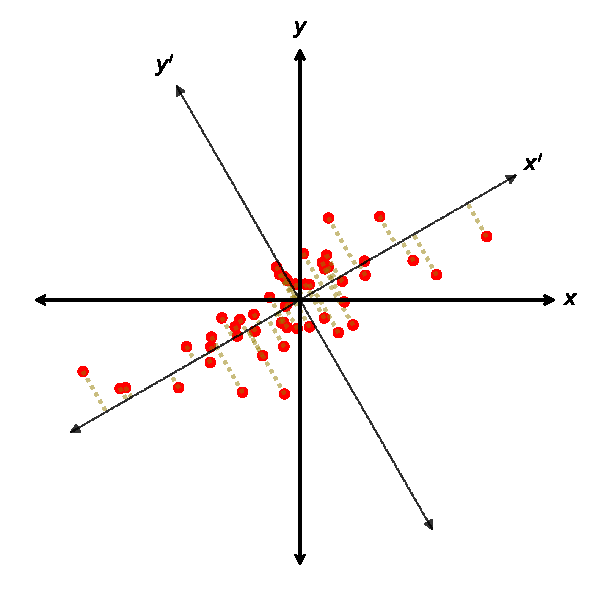
\includegraphics[width=\textwidth]{imagens/pca1.pdf}
    \end{subfigure}
    \begin{subfigure}[t]{0.48\textwidth}
    \caption{Apenas 1\textordmasculine componente principal}
    \centering
    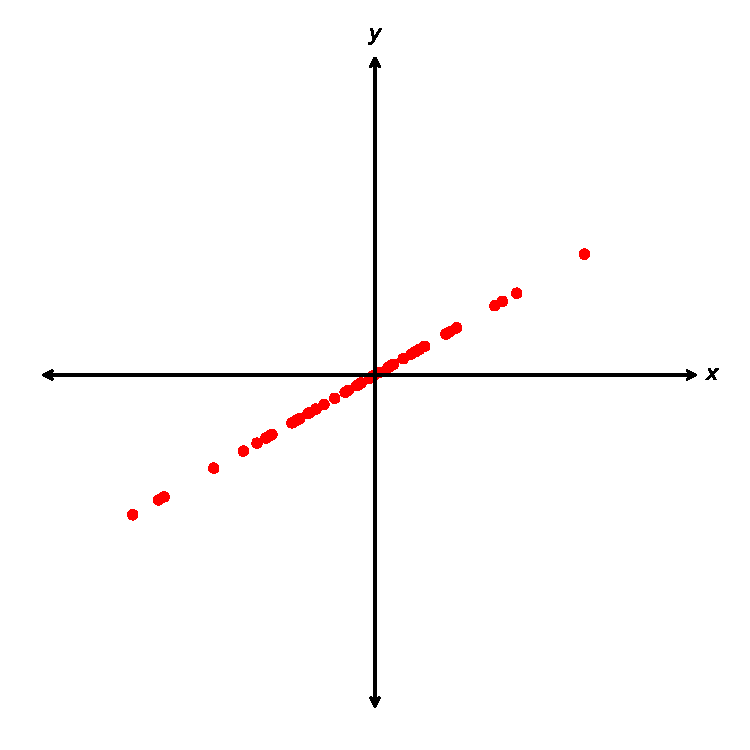
\includegraphics[width=\textwidth]{imagens/pca2.pdf}
    \end{subfigure}
\end{figure}
\end{frame}

%SUBSEC%%%%%%%%%%%%%%%%%%%%%%%%%%%%%%%%%%%%%%%%%%%%%%%
\subsection{Eigenfaces}

%FRAME%%%%%%%%%%%%%%%%%%%%%%%%%%%%%%%%%%%%%%%%%%%%%%%
\begin{frame}{Eigenfaces}
\begin{itemize}
    \item Método desenvolvido por \citeonline{turk1991eigenfaces}
    \item Eigenfaces são os componentes principais de uma distribuição de faces
    \item Cada face pode ser representada como uma combinação linear de eigenfaces
\end{itemize}
\begin{figure}[htbp]
    \centering
%    \caption{Representação de uma face como combinação linear de eigenfaces}
    \label{fig:eigenfaces_comblinear}
    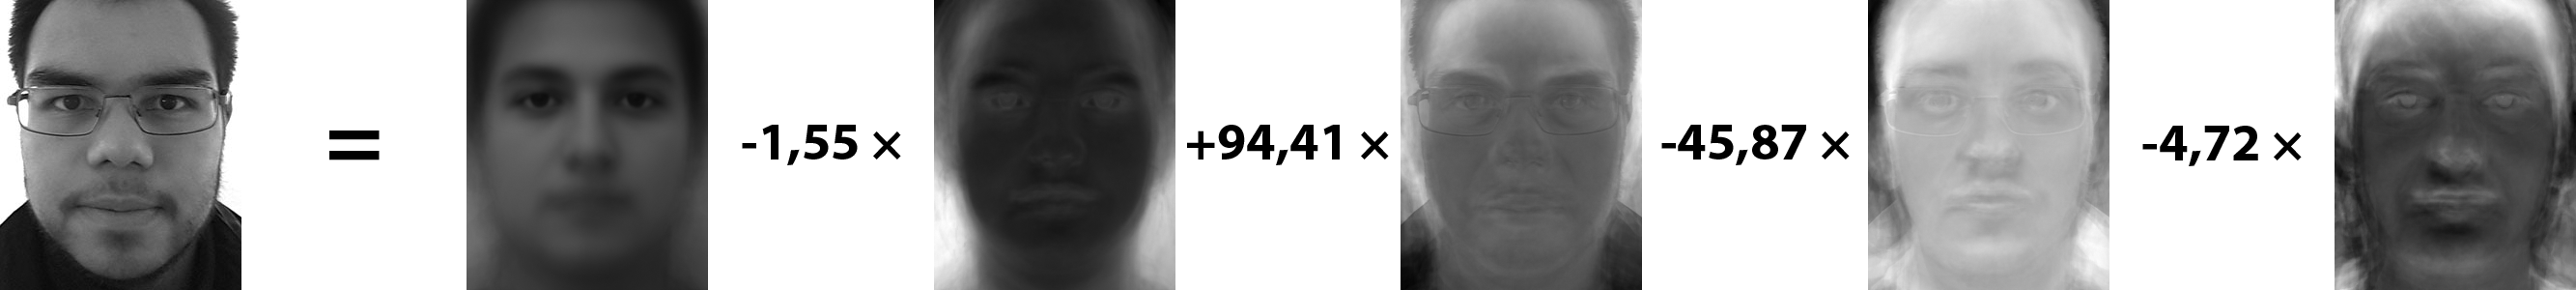
\includegraphics[width=0.95\linewidth]{imagens/eign_lincomb.png}
\end{figure}
\end{frame}


%FRAME%%%%%%%%%%%%%%%%%%%%%%%%%%%%%%%%%%%%%%%%%%%%%%%
\begin{frame}{Eigenfaces}
Algoritmo:
\begin{enumerate}
    \item Obter $M$ imagens $I_1, I_2, I_3 \ldots I_M$ com dimensão $N \times N$.
    As imagens devem estar centralizadas.
    \item Representar cada imagem $I_i$ como um vetor $\Gamma_i$ de dimensão $N^2 \times 1$.
    %
    \begin{equation*} \label{eq:eign_gamma}
        \begin{bmatrix}
        a_{11} & a_{12} & \cdots & a_{1N}\\ 
        a_{21} & a_{22} & \cdots & a_{2N}\\ 
        \vdots & \vdots & \ddots & \vdots\\ 
        a_{N1} & a_{N1} & \cdots & a_{NN}
        \end{bmatrix}_{N \times N} \rightarrow \begin{bmatrix}
        a_{11}\\ 
        \vdots\\ 
        a_{1N}\\ 
        \vdots\\ 
        a_{2N}\\
        \vdots\\ 
        a_{NN}
        \end{bmatrix}_{N^2 \times 1}
    \end{equation*}
    %
    \seti
\end{enumerate}
\end{frame}


%FRAME%%%%%%%%%%%%%%%%%%%%%%%%%%%%%%%%%%%%%%%%%%%%%%%
\begin{frame}{Eigenfaces}
\begin{enumerate}
    \conti
    \item Calcular o vetor $\Psi$ correspondente à face média.
    %
    \begin{equation*} \label{eq:eign_media}
        \Psi = \frac{1}{M}\sum_{i=1}^{M}\Gamma_i
    \end{equation*}
    %
    \item Subtrair a face média de cada vetor $\Gamma_i$ para obter o conjunto de vetores $\Phi_i$.
    %
    \begin{equation*} \label{eq:eign_phi}
        \Phi_i = \Gamma_i - \Psi
    \end{equation*}
    %
    \item Encontrar a matriz $C$ de covariância.
    %
    \begin{equation*} \label{eq:eign_c}
        C = AA^T \text{, onde } A = \begin{bmatrix}\Phi_1  & \Phi_2 & \ldots  & \Phi_3\end{bmatrix}
    \end{equation*}
    %
    $C$ é uma matriz $N^2 \times N^2$ e $A$ é uma matriz $N^2 \times M$.
    \seti
\end{enumerate}
\end{frame}


%FRAME%%%%%%%%%%%%%%%%%%%%%%%%%%%%%%%%%%%%%%%%%%%%%%%
\begin{frame}{Eigenfaces}
\begin{enumerate}
    \conti
    \item Calcular os autovetores $u_i$ de $C = AA^T$.
    
    Em vez desse cálculo, que resultaria em $N^2$ autovetores, calcular os autovetores $v_i$ da matriz $A^TA$ de dimensão $M \times M$.
    %
    \begin{equation*} \label{eq:eign_autov}
    \begin{alignedat}{2}
                     && A^T Av_i    &= \mu_i v_i\\
    \Rightarrow\quad && AA^T Av_i   &= \mu_i Av_i\\
    \Rightarrow\quad && CAv_i       &= \mu_i Av_i\\
    \Rightarrow\quad && u_i         &= Av_i
    \end{alignedat}
    \end{equation*}
    %
    ou seja, $Av_i$ são autovetores de $C = AA^T$. Os $M$ autovalores de $A^TA$ correspondem aos $M$ maiores autovalores de $AA^T$.
    \item Manter apenas os $K$ autovetores, correspondentes aos $K$ maiores autovalores.%
    \seti
\end{enumerate}
\end{frame}


%SUBSEC%%%%%%%%%%%%%%%%%%%%%%%%%%%%%%%%%%%%%%%%%%%%%%%
\subsection{OpenCV}

%FRAME%%%%%%%%%%%%%%%%%%%%%%%%%%%%%%%%%%%%%%%%%%%%%%%
\begin{frame}[fragile]{OpenCV}
\begin{minted}[fontsize=\small]{python}
# Obtém imagens de treino com ids e nomes
imgs, ids, nomes = le_imagens_de_treino(dir_treino)

# Treina o reconhecedor de faces
reconhecedor = cv2.face.EigenFaceRecognizer_create(300)
reconhecedor.train(np.asarray(imgs),np.asarray(ids))

# Realiza o reconhecimento
cinza = cv2.imread(foto, cv2.IMREAD_GRAYSCALE)
num, confianca = reconhecedor.predict(cinza)
nome = nomes[num]
\end{minted}
\end{frame}


%FRAME%%%%%%%%%%%%%%%%%%%%%%%%%%%%%%%%%%%%%%%%%%%%%%%
\begin{frame}{Eigenfaces}

\begin{figure}[htbp]
    \centering
%    \caption{Eigenfaces}
    \label{fig:eigenfaces_faces}
    \begin{subfigure}[t]{0.3\textwidth}
    \centering
    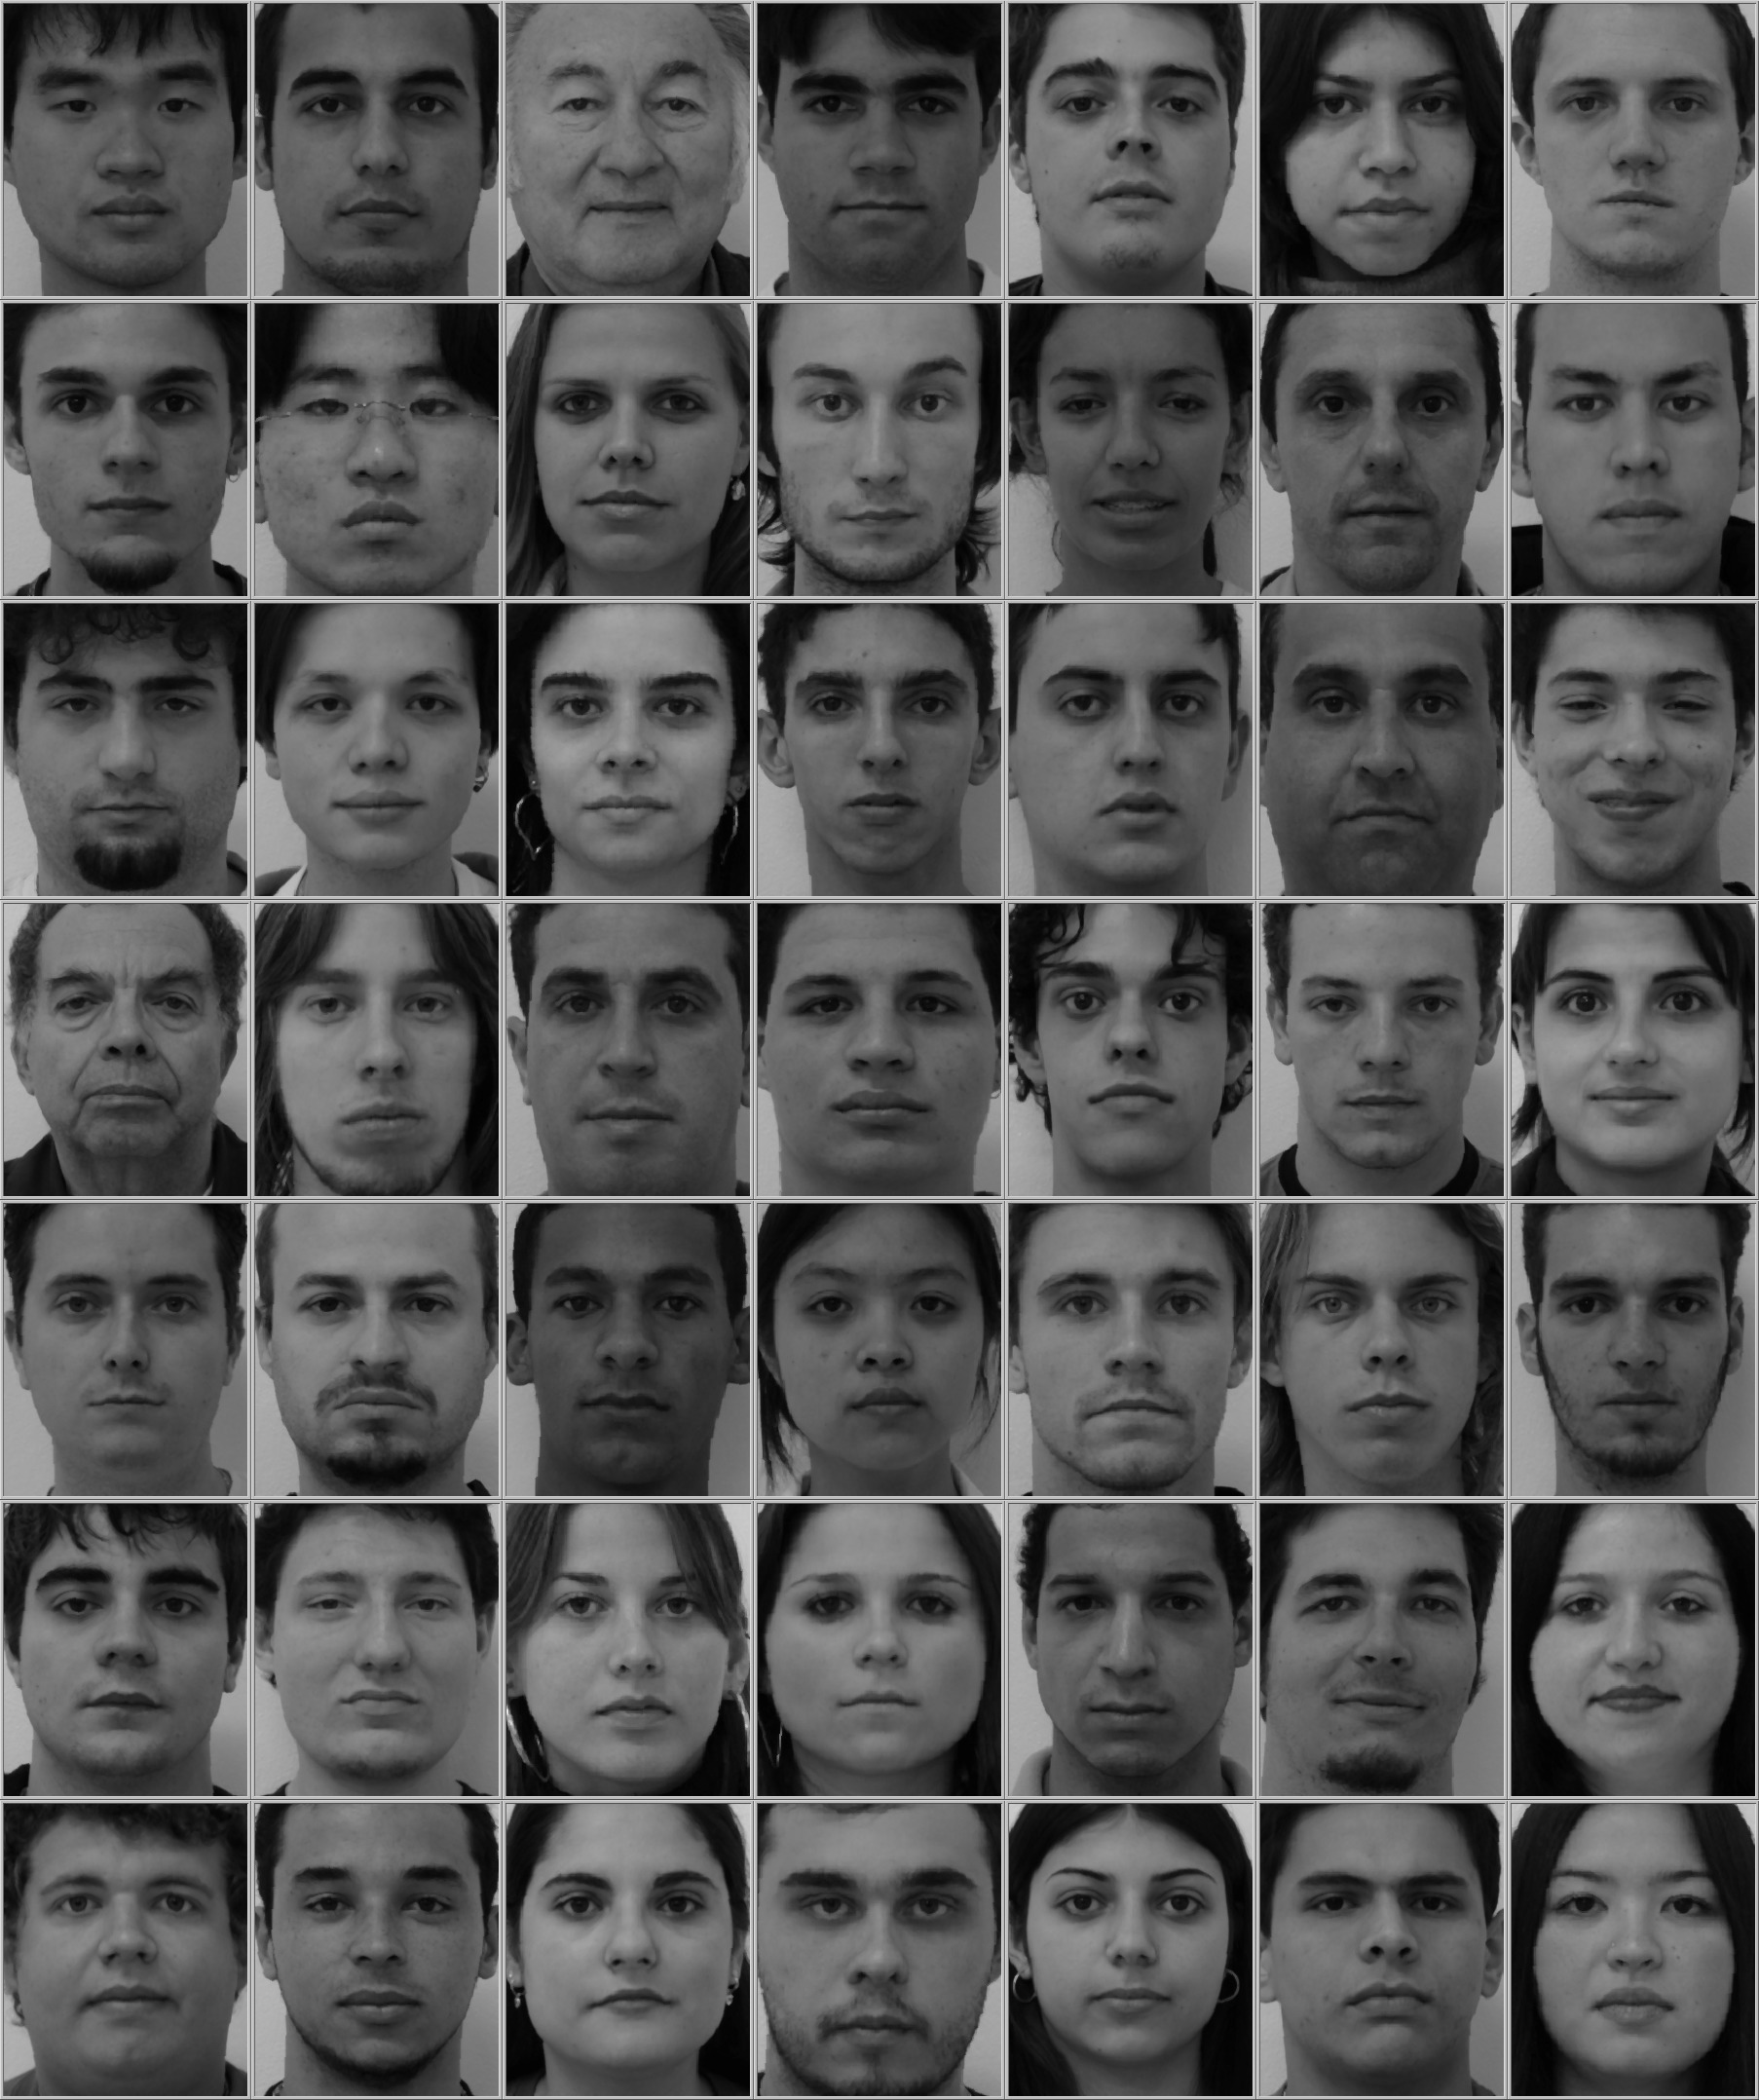
\includegraphics[width=\textwidth]{imagens/faces_fei.jpg}
    \caption{FEI Face Database}
    \end{subfigure}
    \begin{subfigure}[t]{0.3\textwidth}
    \centering
    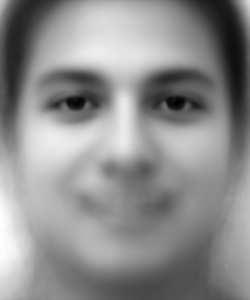
\includegraphics[width=\textwidth]{imagens/face_media.png}
    \caption{Face média}
    \end{subfigure}
    \begin{subfigure}[t]{0.3\textwidth}
    \centering
    
\includegraphics[width=\textwidth]{imagens/eigenfaces.png}
    \caption{Eigenfaces}
    \end{subfigure}
\end{figure}
\end{frame}


%FRAME%%%%%%%%%%%%%%%%%%%%%%%%%%%%%%%%%%%%%%%%%%%%%%%
\begin{frame}{Eigenfaces}
\begin{figure}[htbp]
    \centering
    \caption{Teste com o banco de faces FERET}
    \label{fig:eigenfaces_resultado_feret}
    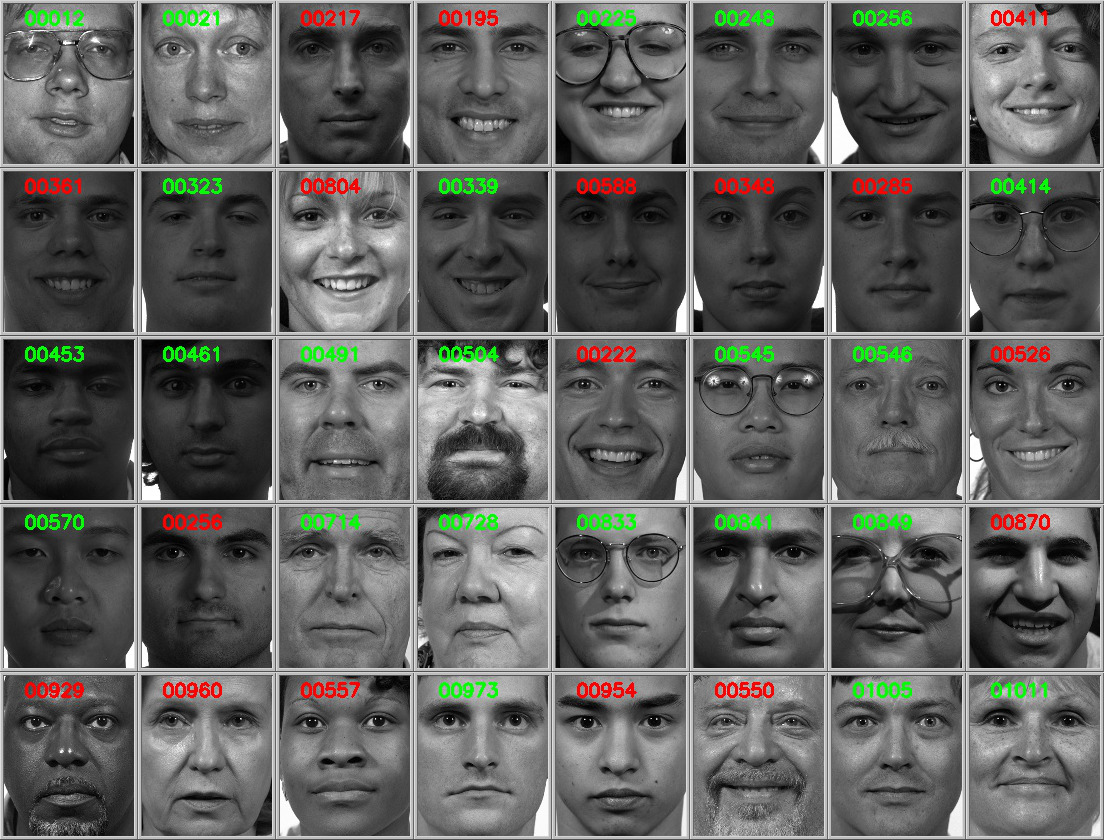
\includegraphics[width=0.8\linewidth]{imagens/eigenfaces_resultado_feret.jpg}
\end{figure}
\end{frame}


%FRAME%%%%%%%%%%%%%%%%%%%%%%%%%%%%%%%%%%%%%%%%%%%%%%%
\begin{frame}{Eigenfaces}
\begin{table}[htpb]
\centering
\caption{Bancos de faces utilizados para testes}
\label{tab:bancos_faces}
\begin{tabular}{|l|l|l|}
\hline
\textbf{Banco de faces} & \textbf{Indivíduos} & \textbf{Fotos de treino} \\\hline
\textbf{AT\&T}          & 40                  & 360                      \\\hline
\textbf{FERET}          & 865                 & 1542                     \\\hline
\textbf{Extended Yale}  & 38                  & 1862                     \\\hline
\end{tabular}
\end{table}
\end{frame}


%FRAME%%%%%%%%%%%%%%%%%%%%%%%%%%%%%%%%%%%%%%%%%%%%%%%
\begin{frame}{Eigenfaces}
\begin{table}[htbp]
\centering
\caption{Comparação dos algoritmos de reconhecimento facial}
\label{tab:compara_reconhecimento}
\begin{tabular}{|c|l|l|}
\hline
\textbf{Método}                       & \textbf{Banco de faces} & \textbf{Taxa de acertos} \\\hline
\multirow{3}{*}{\textbf{Eigenfaces}}  & AT\&T                   & 95,0\%                   \\
                                      & FERET                   & 63,4\%                   \\
                                      & Extended Yale           & 81,6\%                   \\\hline
\multirow{3}{*}{\textbf{Fisherfaces}} & AT\&T                   & 97,5\%                   \\
                                      & FERET                   & -                        \\
                                      & Extended Yale           & 100\%                    \\\hline
\multirow{3}{*}{\textbf{LBPH}}        & AT\&T                   & 100\%                    \\
                                      & FERET                   & 90,7\%                   \\
                                      & Extended Yale           & 94,7\%                   \\\hline
\end{tabular}
\end{table}
\end{frame}